\subsection{Hasil Lokalisasi ICP}

\begin{figure}[H]
\centering
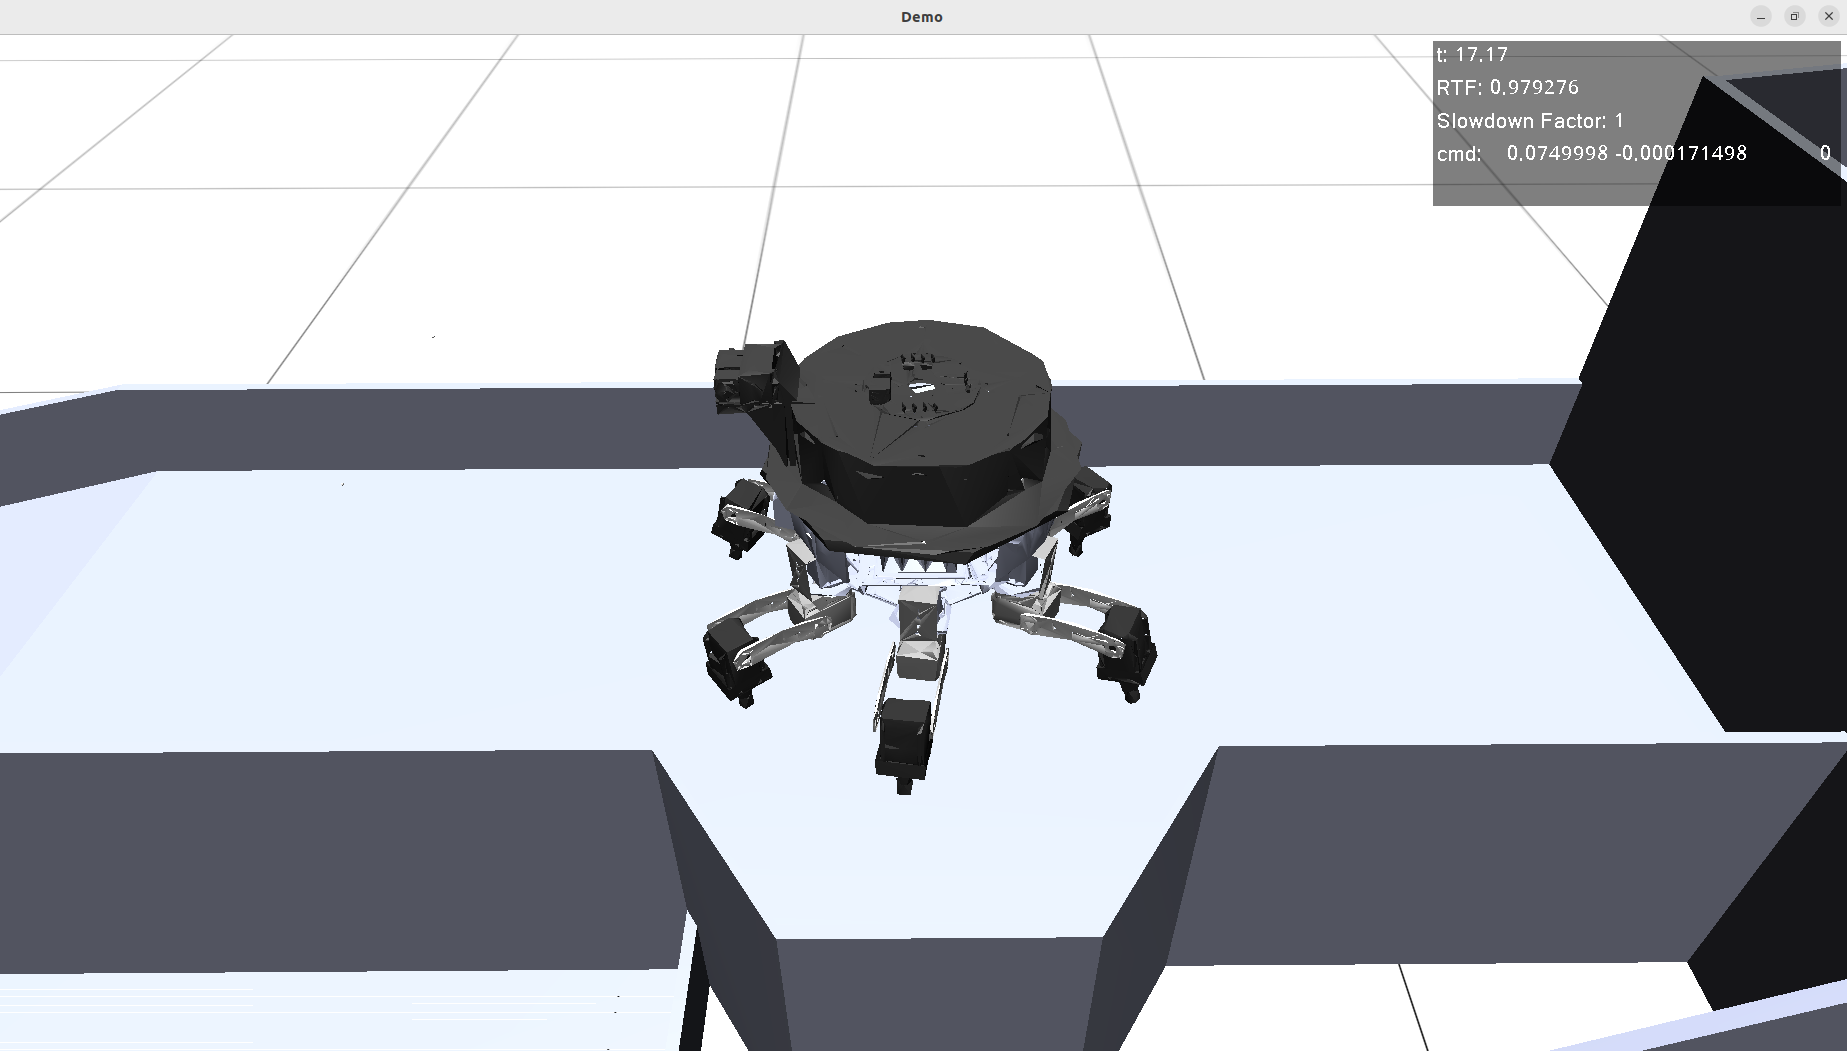
\includegraphics[width=0.7\textwidth]{gambar/sim_RA.png}
\caption{Simulasi di Region A}
\label{fig:sim_ra}
\end{figure}

\begin{figure}[H]
\centering
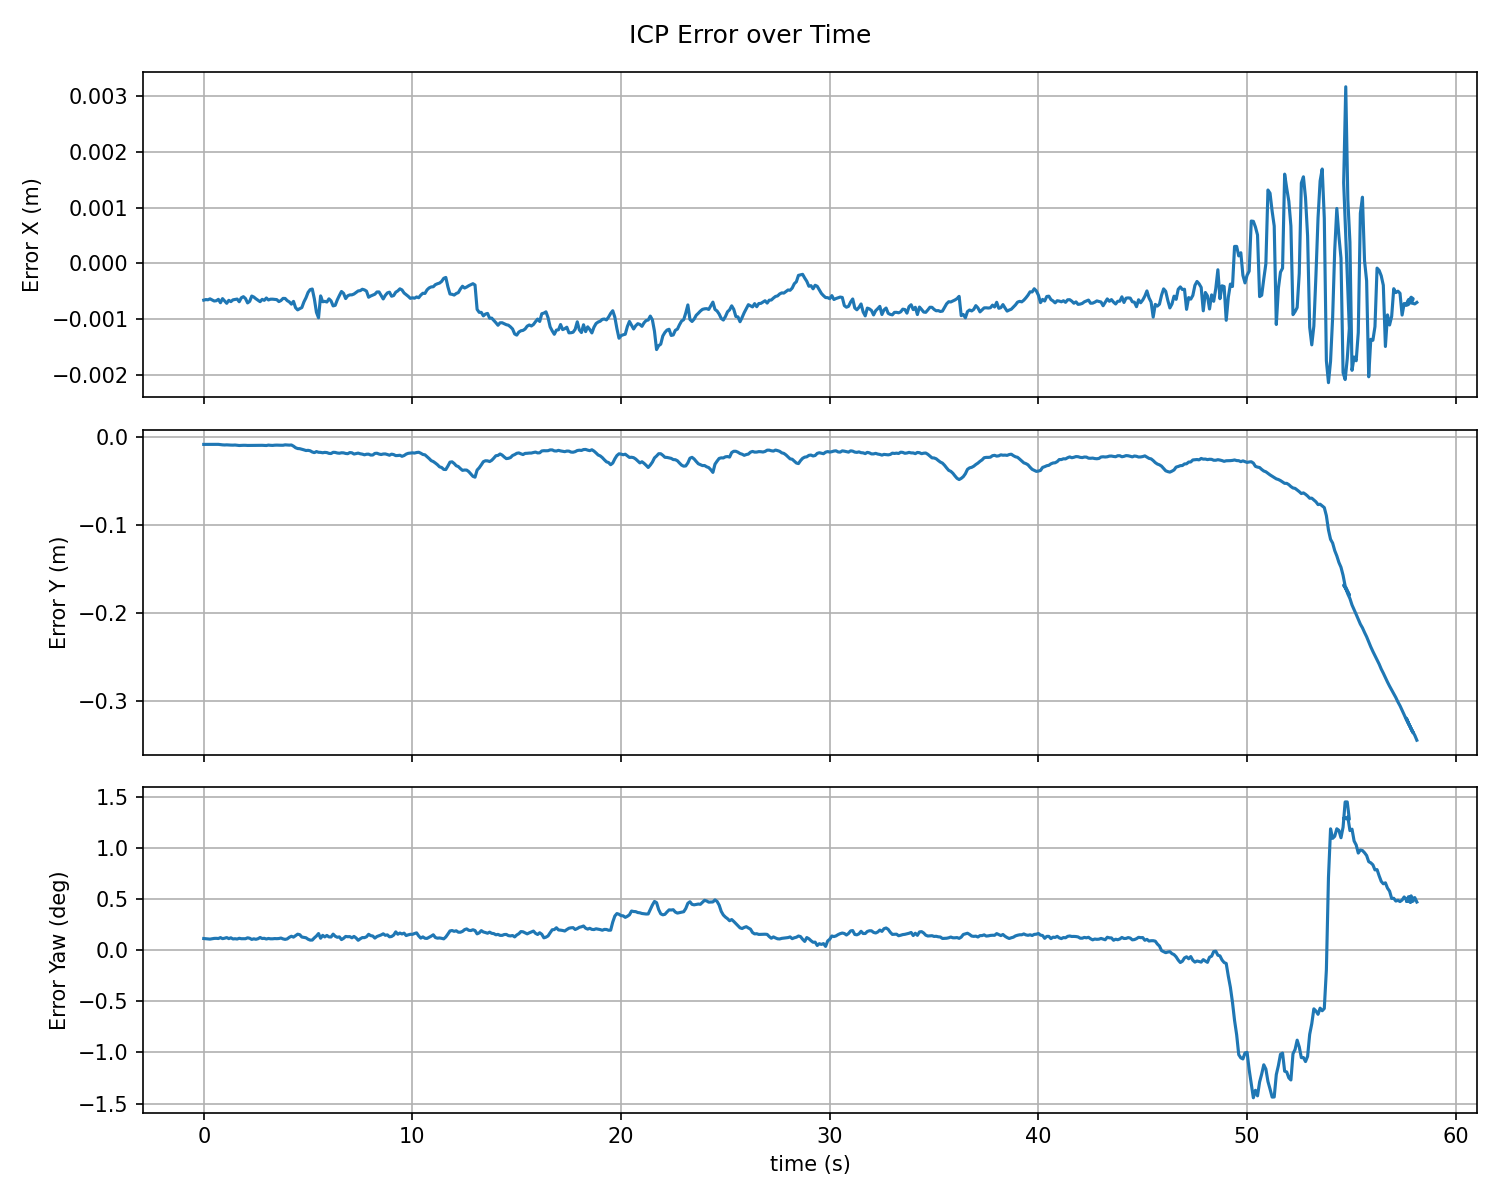
\includegraphics[width=0.9\textwidth]{gambar/icp_errors_RA.png}
\caption{Error ICP di Region A}
\label{fig:icp_errors_ra}
\end{figure}

\begin{figure}[H]
\centering
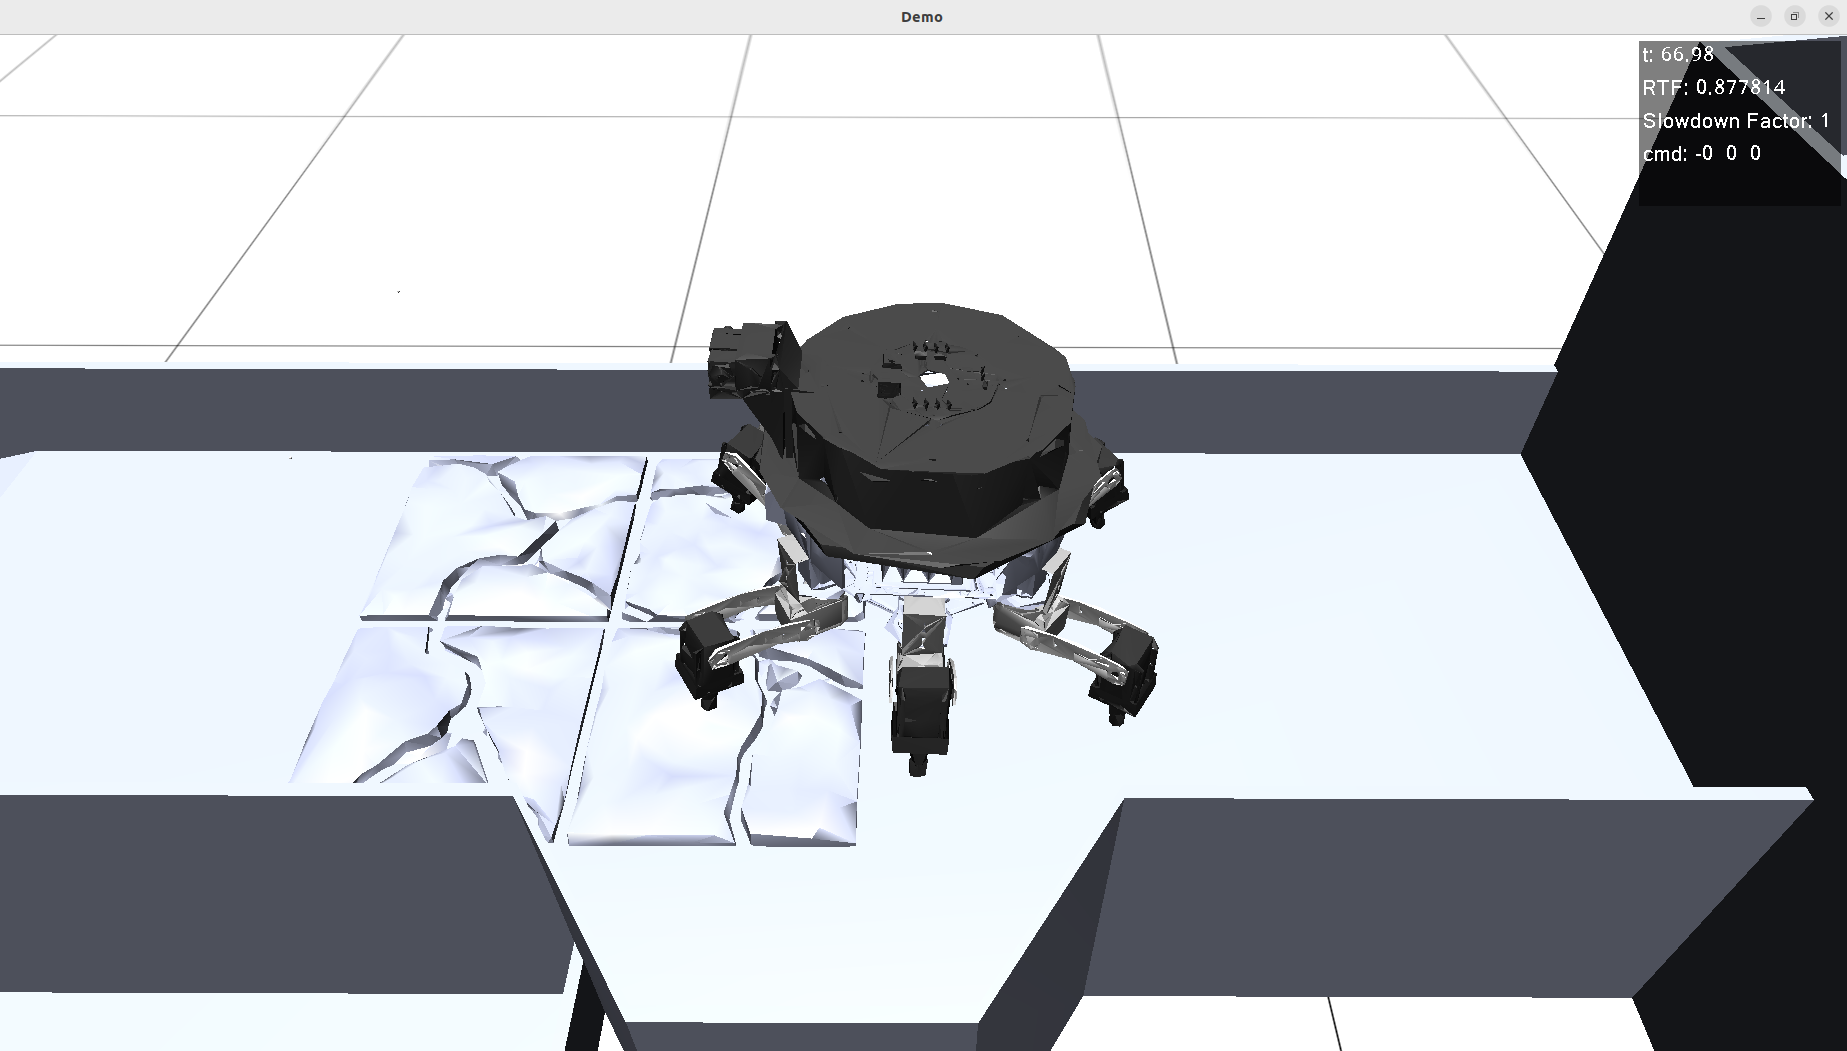
\includegraphics[width=0.7\textwidth]{gambar/sim_RA_rough.png}
\caption{Simulasi di Region A dengan rintangan lantai}
\label{fig:sim_ra_rough}
\end{figure}

\begin{figure}[H]
\centering
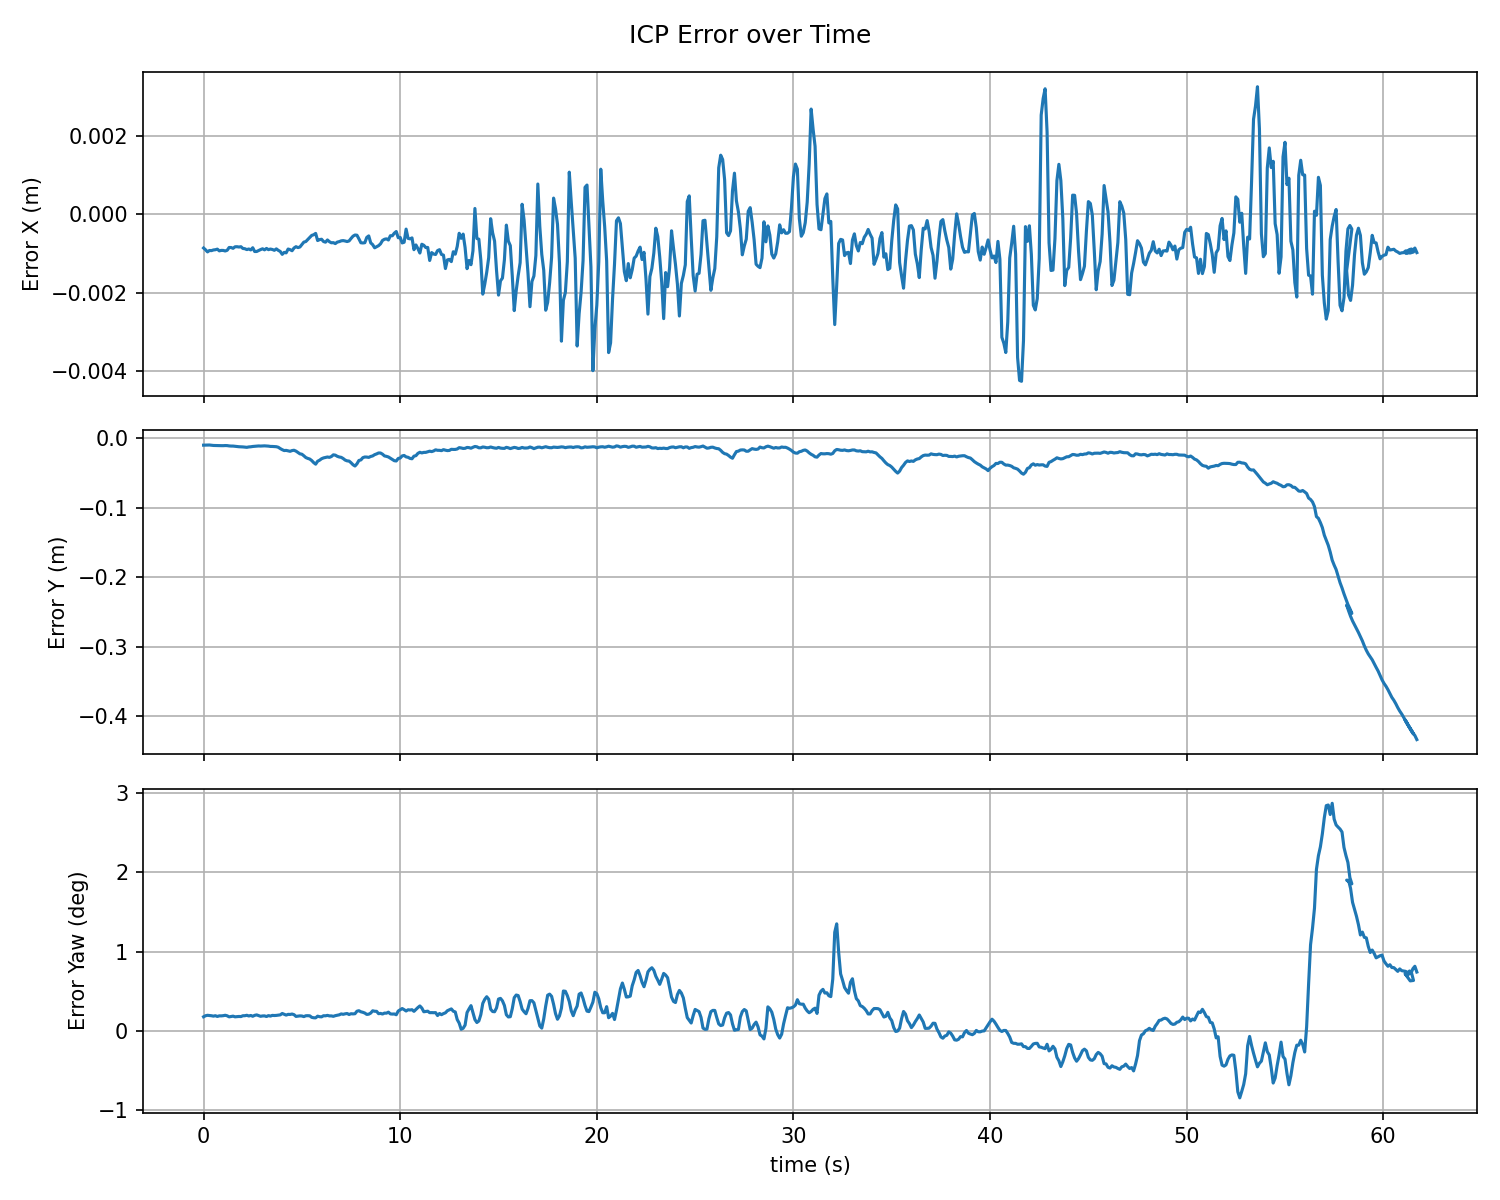
\includegraphics[width=0.9\textwidth]{gambar/icp_errors_RA_rough.png}
\caption{Error ICP di Region A dengan rintangan lantai}
\label{fig:icp_errors_ra_rough}
\end{figure}

\begin{figure}[H]
\centering
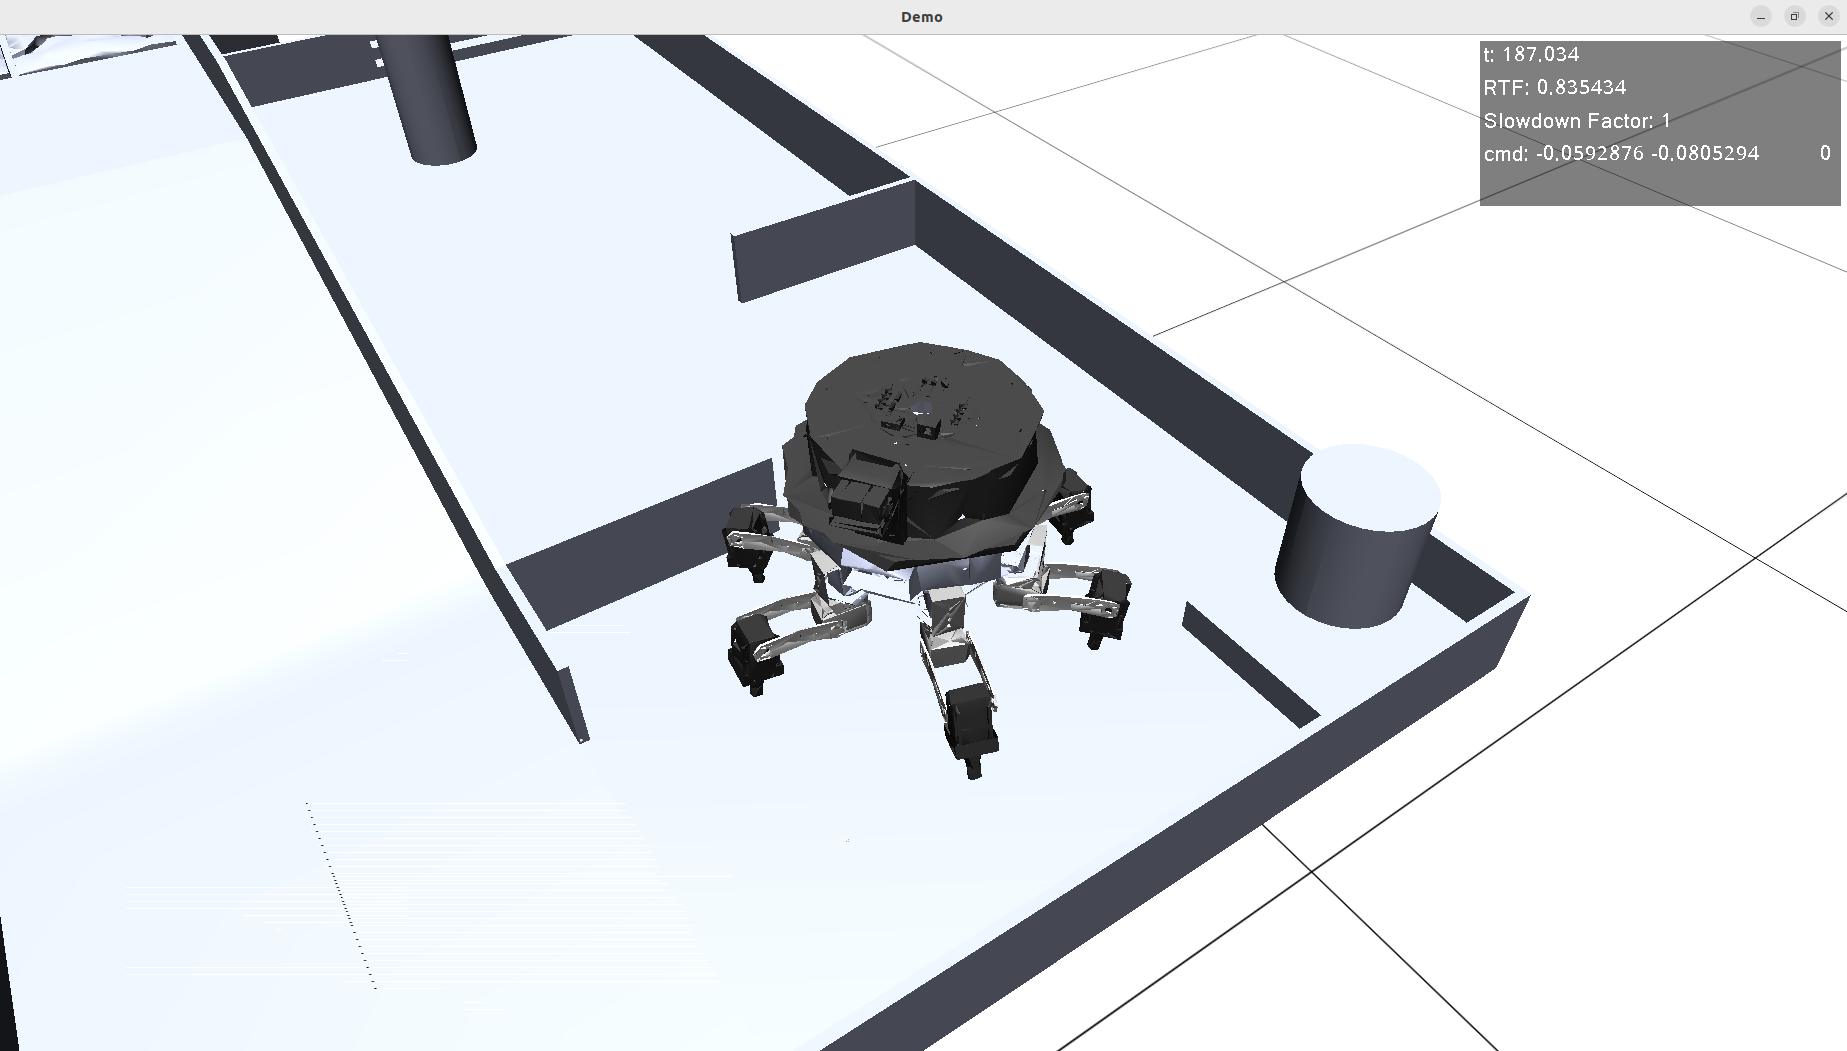
\includegraphics[width=0.7\textwidth]{gambar/sim_RC2.png}
\caption{Simulasi di Region C}
\label{fig:sim_rc2}
\end{figure}

\begin{figure}[H]
\centering
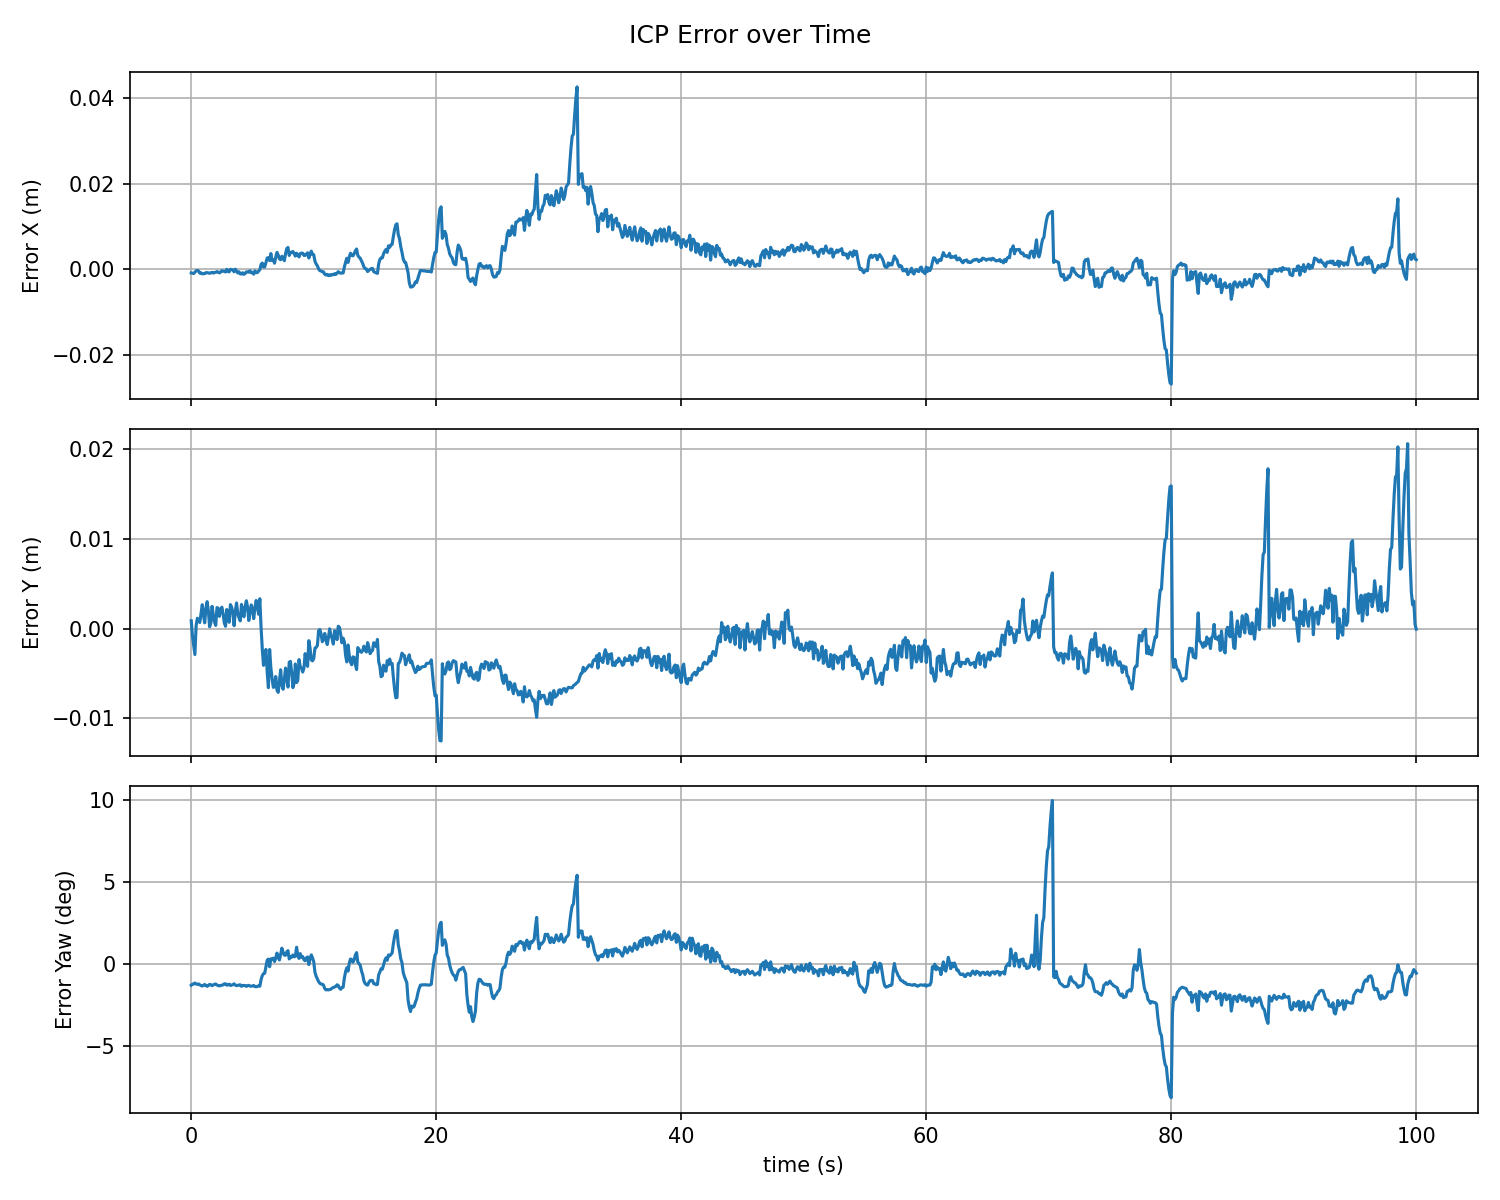
\includegraphics[width=0.9\textwidth]{gambar/icp_errors_RC.png}
\caption{Error ICP di Region C}
\label{fig:icp_errors_rc}
\end{figure}

\subsection{Hasil Global Planner}
\subsubsection{Hasil Path di Region A}

\begin{figure}[H]
\centering
\begin{subfigure}{0.35\textwidth}
    \centering
    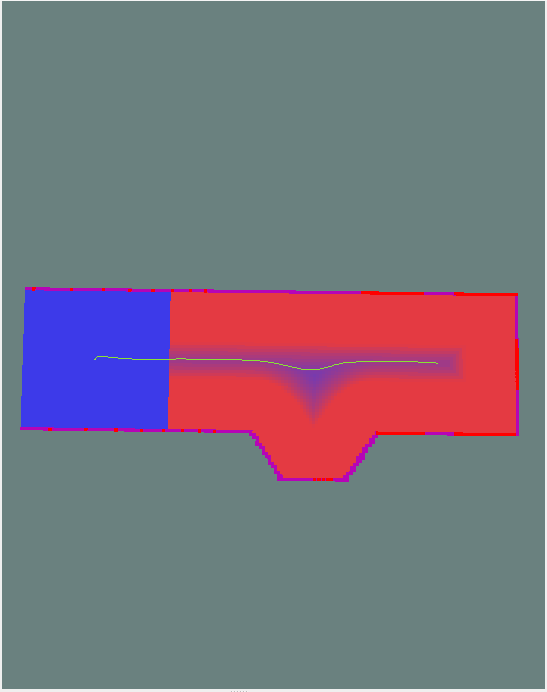
\includegraphics[trim={0 6cm 0 7cm}, clip, width=\textwidth]{gambar/path_CSF10_RA.png}
    \caption{Path dengan CSF 10}
\end{subfigure}
\qquad
\begin{subfigure}{0.35\textwidth}
    \centering
    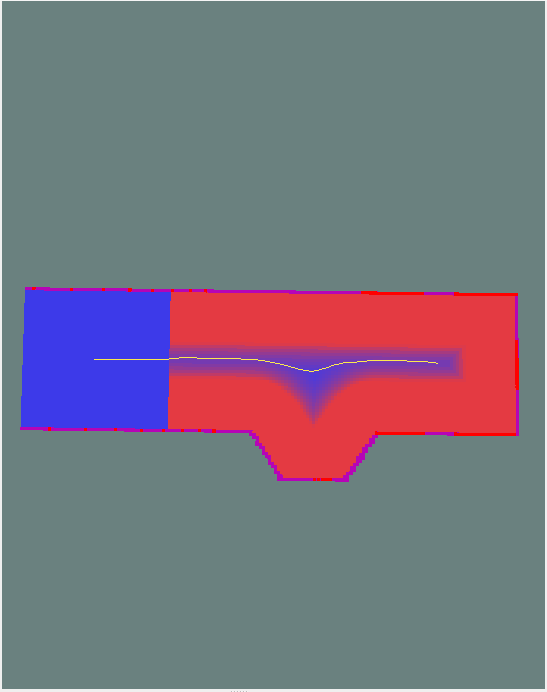
\includegraphics[trim={0 6cm 0 7cm}, clip, width=\textwidth]{gambar/path_CSF20_RA.png}
    \caption{Path dengan CSF 20}
\end{subfigure}
\qquad
\begin{subfigure}{0.35\textwidth}
    \centering
    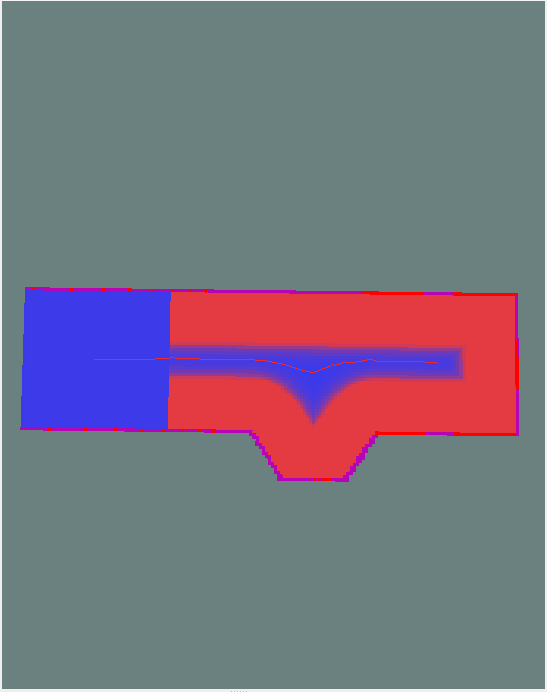
\includegraphics[trim={0 6cm 0 7cm}, clip, width=\textwidth]{gambar/path_CSF50_RA.png}
    \caption{Path dengan CSF 50}
\end{subfigure}
\qquad
\begin{subfigure}{0.35\textwidth}
    \centering
    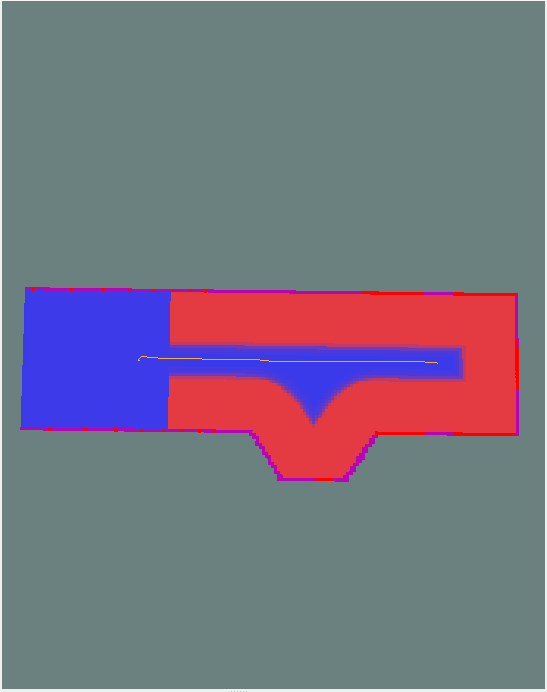
\includegraphics[trim={0 6cm 0 7cm}, clip, width=\textwidth]{gambar/path_CSF100_RA.png}
    \caption{Path dengan CSF 100}
\end{subfigure}
\caption{Relasi path terhadap Cost Scaling Factor di Region A}
\label{fig:path4_RA}
\end{figure}

\begin{table}[H]
\centering
\csvreader[tabular={|c|c|c|c|c|},
           table head={\hline \thead{Cost Scaling\\Factor} & \thead{Panjang\\path (m)} & \thead{Waktu\\komputasi (ms)} & \thead{Min\\clearance (m)} & \thead{Jumlah\\waypoint} \\ \hline},
           late after line={\\\hline}]
  {lampiran/path_CSF_RA.csv}
  {1=\a,2=\b,3=\c,4=\d,5=\e}
  {\a & \b & \c & \d & \e}
\caption{Karakteristik Path di Region A berdasarkan Cost Scaling Factor}
\label{tab:path_csf_ra}
\end{table}

\begin{figure}[H]
\centering
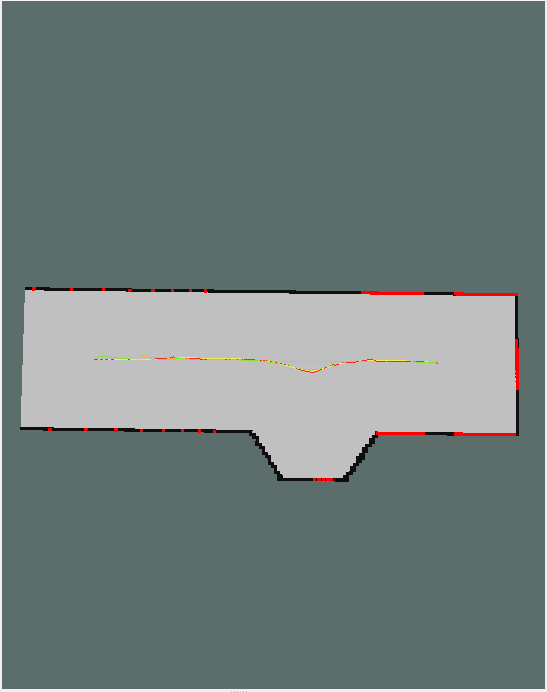
\includegraphics[trim={0 6cm 0 7cm}, clip, width=0.5\textwidth]{gambar/path_all_RA.png}
\caption{Semua path di region A.\\ \textcolor{green}{$\bullet$} CSF 10,\textcolor{yellow}{$\bullet$} CSF 20, \textcolor{red}{$\bullet$} CSF 50, \textcolor{orange}{$\bullet$} CSF 100}
\label{fig:path_all_ra}
\end{figure}

\subsubsection{Hasil Path di Region B}

\begin{figure}[H]
\centering
\begin{subfigure}{0.35\textwidth}
    \centering
    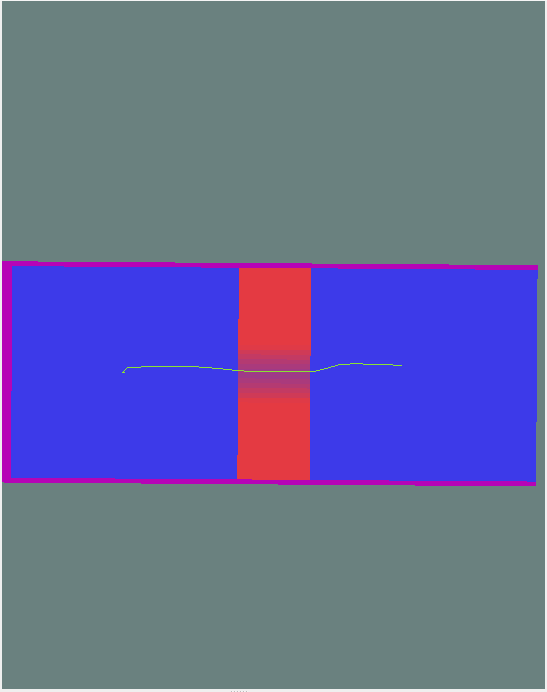
\includegraphics[trim={0 6cm 0 7cm}, clip, width=\textwidth]{gambar/path_CSF10_RB.png}
    \caption{Path dengan CSF 10}
\end{subfigure}
\qquad
\begin{subfigure}{0.35\textwidth}
    \centering
    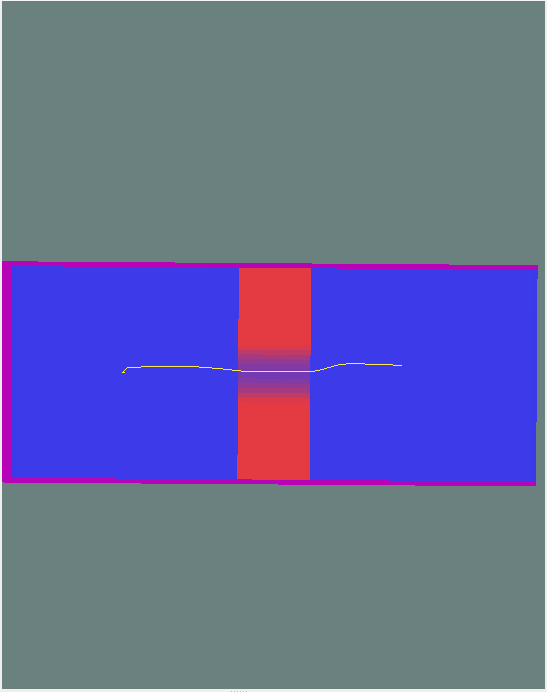
\includegraphics[trim={0 6cm 0 7cm}, clip, width=\textwidth]{gambar/path_CSF20_RB.png}
    \caption{Path dengan CSF 20}
\end{subfigure}
\qquad
\begin{subfigure}{0.35\textwidth}
    \centering
    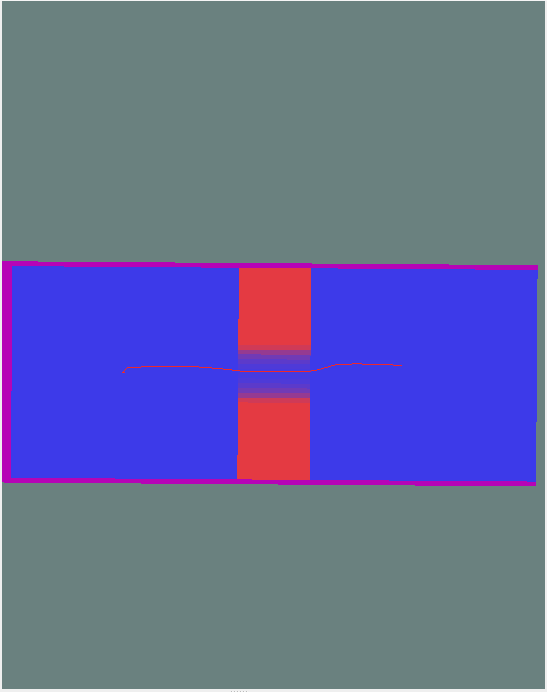
\includegraphics[trim={0 6cm 0 7cm}, clip, width=\textwidth]{gambar/path_CSF50_RB.png}
    \caption{Path dengan CSF 50}
\end{subfigure}
\qquad
\begin{subfigure}{0.35\textwidth}
    \centering
    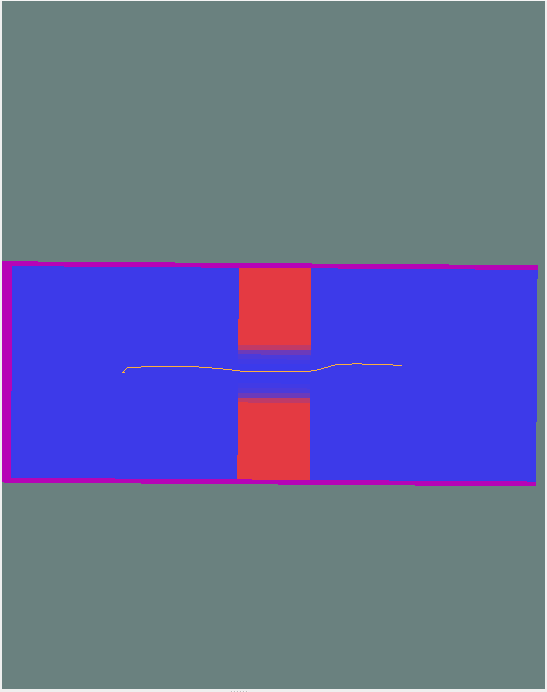
\includegraphics[trim={0 6cm 0 7cm}, clip, width=\textwidth]{gambar/path_CSF100_RB.png}
    \caption{Path dengan CSF 100}
\end{subfigure}
\caption{Relasi path terhadap Cost Scaling Factor di Region B}
\label{fig:path4_RB}
\end{figure}

\begin{table}[H]
\centering
\csvreader[tabular={|c|c|c|c|c|},
           table head={\hline \thead{Cost Scaling\\Factor} & \thead{Panjang\\path (m)} & \thead{Waktu\\komputasi (ms)} & \thead{Min\\clearance (m)} & \thead{Jumlah\\waypoint} \\ \hline},
           late after line={\\\hline}]
  {lampiran/path_CSF_RB.csv}
  {1=\a,2=\b,3=\c,4=\d,5=\e}
  {\a & \b & \c & \d & \e}
\caption{Karakteristik Path di Region B berdasarkan Cost Scaling Factor}
\label{tab:path_csf_rb}
\end{table}

\begin{figure}[H]
\centering
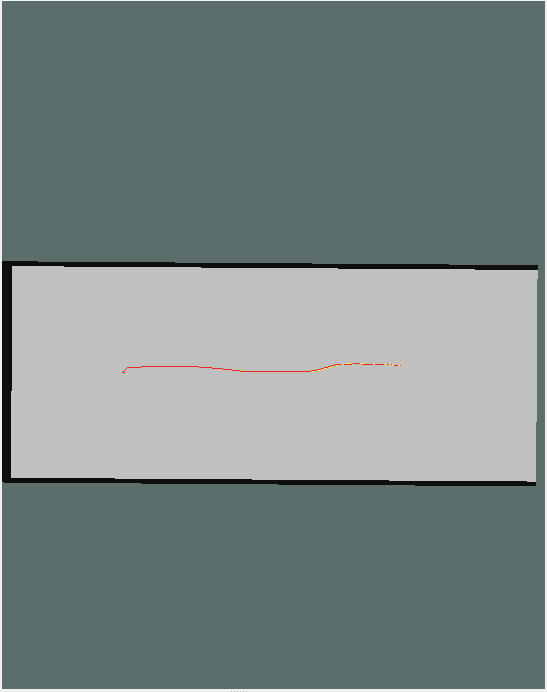
\includegraphics[trim={0 6cm 0 7cm}, clip, width=0.5\textwidth]{gambar/path_all_RB.png}
\caption{Semua path di region B. \\ \textcolor{green}{$\bullet$} CSF 10,\textcolor{yellow}{$\bullet$} CSF 20, \textcolor{red}{$\bullet$} CSF 50, \textcolor{orange}{$\bullet$} CSF 100}
\label{fig:path_all_rb}
\end{figure}

\subsubsection{Hasil Path di Region C}

\begin{figure}[H]
\centering
\begin{subfigure}{0.3\textwidth}
    \centering
    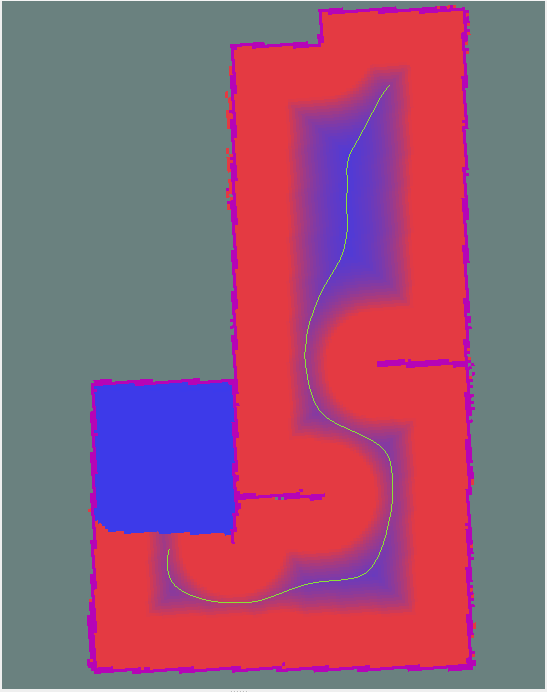
\includegraphics[width=\textwidth]{gambar/path_CSF10_RC.png}
    \caption{Path dengan CSF 10}
\end{subfigure}
\qquad
\begin{subfigure}{0.3\textwidth}
    \centering
    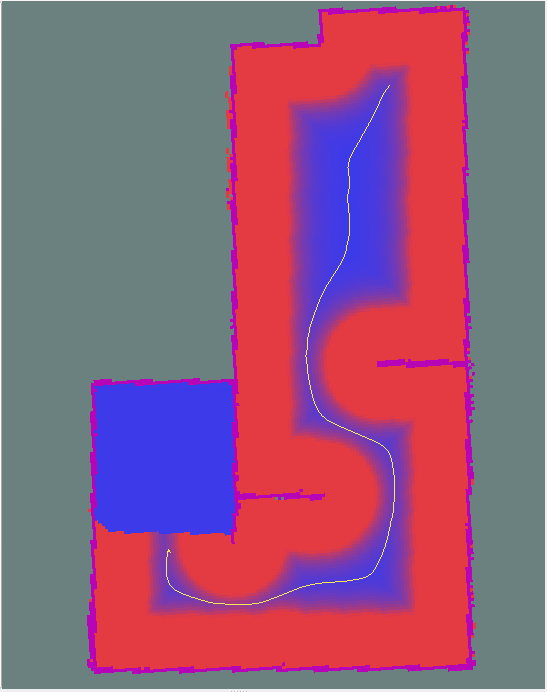
\includegraphics[width=\textwidth]{gambar/path_CSF20_RC.png}
    \caption{Path dengan CSF 20}
\end{subfigure}
\qquad
\begin{subfigure}{0.3\textwidth}
    \centering
    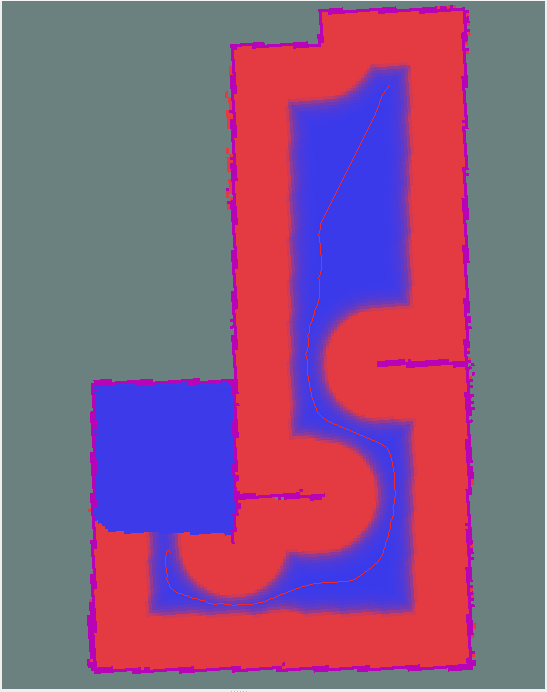
\includegraphics[width=\textwidth]{gambar/path_CSF50_RC.png}
    \caption{Path dengan CSF 50}
\end{subfigure}
\qquad
\begin{subfigure}{0.3\textwidth}
    \centering
    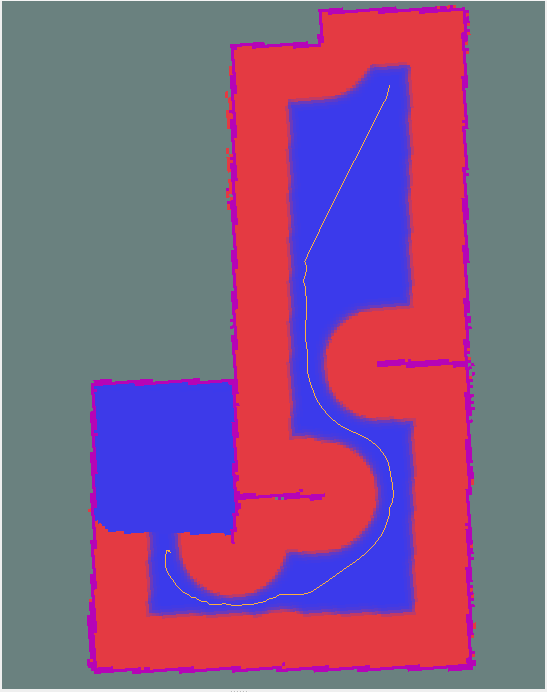
\includegraphics[width=\textwidth]{gambar/path_CSF100_RC.png}
    \caption{Path dengan CSF 100}
\end{subfigure}
\caption{Relasi path terhadap Cost Scaling Factor di Region C}
\label{fig:path4_RC}
\end{figure}

\begin{table}[H]
\centering
\csvreader[tabular={|c|c|c|c|c|},
           table head={\hline \thead{Cost Scaling\\Factor} & \thead{Panjang\\path (m)} & \thead{Waktu\\komputasi (ms)} & \thead{Min\\clearance (m)} & \thead{Jumlah\\waypoint} \\ \hline},
           late after line={\\\hline}]
  {lampiran/path_CSF_RC.csv}
  {1=\a,2=\b,3=\c,4=\d,5=\e}
  {\a & \b & \c & \d & \e}
\caption{Karakteristik Path di Region C berdasarkan Cost Scaling Factor}
\label{tab:path_csf_rc}
\end{table}

\begin{figure}[H]
\centering
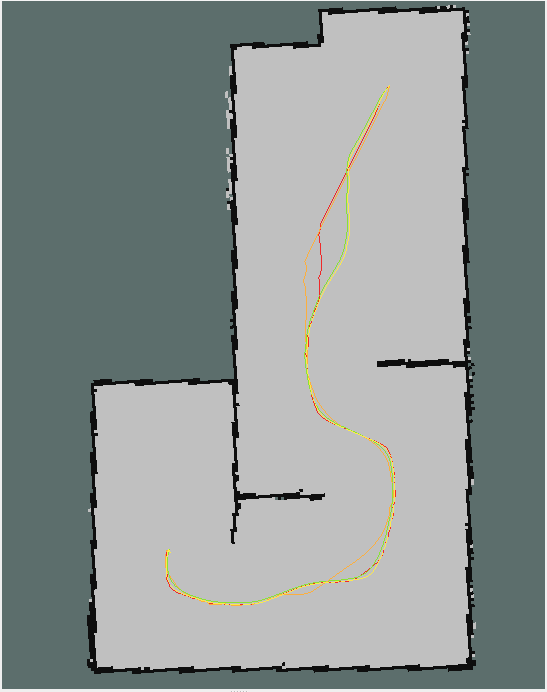
\includegraphics[width=0.5\textwidth]{gambar/path_all_RC.png}
\caption{Semua path di region C.\\ \textcolor{green}{$\bullet$} CSF 10,\textcolor{yellow}{$\bullet$} CSF 20, \textcolor{red}{$\bullet$} CSF 50, \textcolor{orange}{$\bullet$} CSF 100}
\label{fig:path_all_rc}
\end{figure}

\begin{table}[H]
\centering
\csvreader[tabular={|c|c|c|c|c|c|},
           table head={\hline \thead{Cost Scaling\\Factor} & \thead{Rata-rata\\panjang Path (m)} & \thead{Jumlah\\waypoint}  & \thead{Mean cross\\track error (m)} & \thead{Standard\\Deviation (m)} & \thead{Max Cross\\track Error (m)} \\ \hline},
           late after line={\\\hline}]
  {lampiran/path_comparison_RA.csv}
  {1=\a,2=\b,3=\c,4=\d,5=\e,6=\f}
  {\a & \b & \c & \d & \e & \f}
\caption{Perbandingan path terhadap ground truth di region A}
\label{tab:path_comparison_ra}
\end{table}

\begin{table}[H]
\centering
\csvreader[tabular={|c|c|c|c|c|c|},
           table head={\hline \thead{Cost Scaling\\Factor} & \thead{Rata-rata\\panjang Path (m)} & \thead{Jumlah\\waypoint}  & \thead{Mean cross\\track error (m)} & \thead{Standard\\Deviation (m)} & \thead{Max Cross\\track Error (m)} \\ \hline},
           late after line={\\\hline}]
  {lampiran/path_comparison_RB.csv}
  {1=\a,2=\b,3=\c,4=\d,5=\e,6=\f}
  {\a & \b & \c & \d & \e & \f}
\caption{Perbandingan path terhadap ground truth di region B}
\label{tab:path_comparison_rb}
\end{table}

\begin{table}[H]
\centering
\csvreader[tabular={|c|c|c|c|c|c|},
           table head={\hline \thead{Cost Scaling\\Factor} & \thead{Rata-rata\\panjang Path (m)} & \thead{Jumlah\\waypoint}  & \thead{Mean cross\\track error (m)} & \thead{Standard\\Deviation (m)} & \thead{Max Cross\\track Error (m)} \\ \hline},
           late after line={\\\hline}]
  {lampiran/path_comparison_RC.csv}
  {1=\a,2=\b,3=\c,4=\d,5=\e,6=\f}
  {\a & \b & \c & \d & \e & \f}
\caption{Perbandingan path terhadap ground truth di region C}
\label{tab:path_comparison_rc}
\end{table}